\graphicspath{{/Users/brunomedina/Dropbox/Tesis-Egobets/egobets-notas/resources/marco/}}
\chapter{Marco teórico}
\section{Ligas europeas de futbol}
El nivel de juego de los clubes europeos es sorprendente, tanto en la cancha como fuera de ella los Clubes de futbol de las ligas europeas hacen las cosas mejor que ningún otro. Ofrecen partidos de alta calidad, con jugadas complejas y rápidas que proveen de un espectáculo como ningún otro. Además de que la infraestructura, adminsitración y los recursos financieros con los que cuentan son envidiables. Y es por estos motivos que sus niveles de audiencia y la cantidad de sus fanáticos han llegado a niveles impresionantes. Las ligas europeas son en el mundo del futbol: \emph{El modelo a seguir.}


Además de todas las cualidades con las que cuentan estas ligas, se tiene una premisa muy interesante incita el enfoque en ellas: La consistencia que tienen los equipos más populares de cada liga para conseguir victorias sobre los equipos más modestos y su habilidad para siempre permanecer en los mejores lugares de la tabla de posiciones. 

\subsection{Bundesliga (Alemania)}


Fundada el 28 de Julio de 1962 en la convención anual de la \emph{DFL Deutsche Fußball Liga GmbH}, la primer temporada se jugó en 1963. La liga evolucionó en función de la reunificación de Alemania y la integración de la liga del Este\cite{hesse2003tor} Hoy en día la \emph{Bundesliga} es conocida como una de las ligas con mayor afluencia en sus partidos, en la temporada 2011/12 hubo un promedio de 44,293 espectadores por partido. Se vendieron 18.8 millones de entradas en total.

\begin{figure}[!htb]\centering
   \begin {minipage}{0.4\textwidth}
     
\includegraphics[width=\linewidth]{logo-bundesliga}
   \end{minipage}
\end{figure}
\begin{chapquote}{Gary Lineker, \textit{ex-futbolista inglés.}}
	``El fútbol es un deporte que inventaron los ingleses, que lo saben jugar los brasileños y en el que siempre ganan los alemanes.''
\end{chapquote}


La \emph{DFL} se encarga de la operación de las ligas de futbol: \emph{Bundesliga} y \emph{2. Bundesliga}; que son las más importantes de Alemania. Cuenta con treinta y seis clubs de futbol los cuales juegan se dividen en ambas divisiones (Ver~\cref{sec:equipos-ger}) Todos miembros de la Asociación  de la Liga cuentan con una licencia\footnote{Cada temportada todos los clubs deben cumplir los criterios deportivos, legales, administrativos, financieros y de infraestructura del Lizenzierungsordnung (LO) y sus respectivos apéndices} para poder jugar y deben seguir los sistemas de entrenamiento y procedimientos disciplinarios.

Dieciocho equipos juegan en cada división, cada equipo juega una vez de local y otra de visitante contra cada uno de los otros diecisiete equipos de la liga. Esto significa que al ser $n=18$ equipos se tienen $\sum\limits_{i=1}^{n-1} i= \sum\limits_{i=1}^{17} i= 153 $ partidos en una temporada. Al término de estos partidos se calculan los puntos que cada equipo tiene y se hace la tabla de posiciones, los dos peores equipos de la \emph{Bundesliga} son intercambiados con los dos mejores de la \emph{2. Bundesliga}. Mientras que el tercer mejor equipo de la \emph{2. Bundesliga} disputa un partido con el tercer peor equipo de la \emph{Bundesliga} para decidir quien se queda en la primera división. Análogamente, el equipo con más puntos se vuelve el campeón de la liga.

Los puntos de la tabla son dados por las victorias de cada equipo, una victoria suma tres puntos a la tabla; las derrotas o empates no suman nada. Si en la tabla hay equipos con la misma cantidad de puntos, para el desempate se deben consideran criterios como: diferencias de goles, cantidad de goles anotados en la temporada,  diferencia de goles que resulten de los partidos jugados entre ellos y la cantidad de goles como visitantes. Si todos estos criterios no deciden el desempate, se deberá jugar un partido en una cancha neutral para decidir su posición en la tabla.

La regulación de la cantidad de jugadores extranjeros en los equipos sigue la regulación d ela UEFA desde el 21 de Diciembre del 2005. Actualmente hay 977 jugadores con un contrato profesional, 503 en la \emph{Bundesliga} y 474 en la \emph{2. Bundesliga}. El cuarenta y siete por ciento de la primera división son extranjeros (234 jugadores) y el treinta y seis por ciento  en la segunda liga (171 jugadores)

En total, 43 clubs han ganado la Bundesliga desde su fundación. Los tres equipos con más campeonatos son: \emph{FC Bayern Munich} con 23 títulos, \emph{BFC Dynamo Berlin} con 10 y \emph{1. FC Nürnberg} con 9. Los tres máximos goleadores de la liga son: \emph{Ger Müller} (1965-1979) con 365 goles, \emph{Klaus Fischer} (1968-1988) con 268 y \emph{Jupp Heyncke}s con 220.\cite{bundesliga}

\subsection{Liga BBVA (España)}

La Primera División de España comenzó a disputarse en la temporada 1928-29, siendo el FC. Barcelona el primer equipo que se proclamó Campeón. Hasta ese momento, el fútbol español se organizaba en torno al Campeonato de España. Las primeras temporadas se disputaron con los primeros campeones y subcampeones del Campeonato de España. Conocida hoy en día como la \emph{Liga BBVA}\footnote{Nombre proveniente del patrocinio del Banco Bilbao Vizcaya Argentaria. Segunda División ahora se conoce como la \emph{Liga Adelante}. Curiosamente la Segunda División solía tener el nombre de \emph{Liga BBVA} } (por motivos de patrocinio, es considerada hoy en día como la liga de más fuerte del mundo y de mayor importancia.\cite{strongest-league}

\begin{figure}[!htb]\centering
   \begin {minipage}{0.5\textwidth}
     
\includegraphics[width=\linewidth]{logo-bbva}
   \end{minipage}
\end{figure}

La Liga de Fútbol Profesional (LFP) se fundó el 26 de julio de 1984. Es una asociación deportiva integrada por todas las sociedades anónimas deportivas y clubes de fútbol de Primera y Segunda División que participan en competiciones oficiales profesionales de España. La LFP forma parte de la Real Federación Española de Fútbol pero tiene autonomía jurídica en su organización y funcionamiento. 

En la actualidad, la Liga de Fútbol Profesional está formada por un total de 42 equipos: 20 en Primera División y 22 en Segunda División (Ver~\cref{sec:equipos-esp}). Igual que la liga Alemana, cada equipo juega una vez de local y otra de visitante contra cada uno de los otros diecinueve equipos de la liga. Esto significa que al ser $n=19$ equipos se tienen 190 partidos en una temporada. Con estas 38 jornadas los equipos suman puntos en la tabla de posiciones, los primeros 3 entran a la fase de grupos de la \emph{Liga de Campeones de la UEFA}. Los últimos tres equipos en la tabla de posiciones descienden a la \emph{Liga Adelante}, mientras que los mejoes 2 de la Segunda División suben a Primera. El tercer ascenso a Liga BBVA es el ganador de un mini torneo entre el tercer vs quinto y cuarto vs sexto mejor clasificados.

Cada victoria suma tres puntos al Club vencedor, en caso de empate ambos equipos se llevan un punto. Las reglas de desempate son las siguientes: 
\begin{itemize}

	\item El que tenga una mayor diferencia entre goles a favor y en contra según el resultado de los partidos jugados entre ellos.

	\item El que tenga la mayor diferencia de goles a favor teniendo en cuenta todos los obtenidos y recibidos en el transcurso de la competición.

	\item El club que haya marcado más goles.

\end{itemize}

En caso de que haya tres equipos o más empatados se siguen los siguientes criterios para el desmpate:

\begin{itemize}

	\item La mejor puntuación de la que a cada uno corresponda a tenor de los resultados de los partidos jugados entre sí por los clubes implicados.

	\item La mayor diferencia de goles a favor y en contra, considerando únicamente los partidos jugados entre sí por los clubes implicados.

	\item La mayor diferencia de goles a favor y en contra teniendo en cuenta todos los encuentros del campeonato.

	\item El mayor número de goles a favor teniendo en cuenta todos los encuentros del campeonato.

	\item El club mejor clasificado con arreglo a los baremos de fair play.

\end{itemize}

Se inscriben 25 jugadores cada temporada a cada Club, de los que 3 pueden ser ajenos a la Unión Europea. Sin embargo, todos aquellos que se puedan nacionalizar por sus lazos familiares pueden jugar en el equipo sin ocupar una plaza de extracomunitaria.

59 equipos han jugado en esta ligas desde su comienzo. Los únicos 3 que nunca han descendido son: Athletic Club, FC Barcelona y Real Madrid CF. Los campeones máximos son \emph{Real Madrid CF} con 32 títulos, \emph{FC Barcelona} con 22 y \emph{Club Atlético Madrid} con 10. Loa goleadores más prolíficos son: \emph{Telmo Zarra} (1921-2006) con 251 goles, \emph{Lionel Messi} (1987) con 250 y \emph{Hugo Sánchez} (1958) con 234.\cite{primera}

\subsection{Ligue 1 (Francia)}

Fundada el 11 de septiembre de 1932 bajo el nombre de \emph{National} que después cambió a \emph{Division 1}

\begin{figure}[!htb]\centering
   \begin {minipage}{0.5\textwidth}
     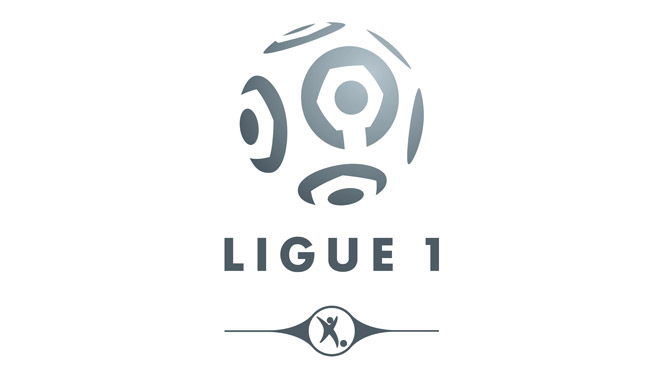
\includegraphics[width=\linewidth]{logo-ligue1}
   \end{minipage}
\end{figure}


\subsection{Premier (Inglaterra)}

La \emph{DFL Deutsche Fußball Liga GmbH} se encarga de la operación de la \emph{Bundesliga} y \emph{2. Bundesliga}, las más importantes ligas de futbol de alemania. Cuenta con treinta y seis clubs 


\subsection{Serie A (Italia)}

La \emph{DFL Deutsche Fußball Liga GmbH} se encarga de la operación de la \emph{Bundesliga} y \emph{2. Bundesliga}, las más importantes ligas de futbol de alemania. Cuenta con treinta y seis clubs 


\section{Apuestas}
Las apuestas han sido por siempre favorecidas en el estudio de las Matemáticas especialmente en áreas tan relacionadas como la probabilidad y la estadística.
Problemas famosos como \emph{La Ruina del Jugador}\cite[p.~95-99]{ross2006first} han sido estudiado desde tiempos de Christian Huygens y Fermat. Gracias a estudios como estos, se hace claro que la casa siempre gana; pero también se puede calcular un tiempo promedio de la duración de los juegos.


\section{Internet}
La era de la información nos golpeo tan fuerte, que ahora es imposible la vida sin nuestros sistemas de información y nuestros dispositivos de conexión. Gracias a las computadoras y las redes, hemos redefinido nuestra imaginación, hemos creado un espacio que expande nuestra mente y nuestra capacidad, nuestras barreras se han alejado más y ahora nuestra conciencia como especie humana, crece en tasas inimaginables. Los monopolios de la información se han ido disolviendo, permitiendo a la sociedad una mayor participación y voz.

Internet es un organismo vivo y hambriento, con el que convivimos de manera simbiótica y nos une como especie. Es un espacio de comunicación y entendimiento. Nunca pudo haber existido algo más majestuoso y poderoso. La verdadera trascendencia del ser, vendrá con la evolución de la conciencia de la sociedad.

